\chapter{Анализ предметной области} \label{chapt1}

\section{Введение в дифференциальный GPS и RTK} \label{sect1_1}

Дифференциальный GPS подразумевает использование двух приемников для улучшения качества получаемых координат. Один из них, называемый \textbf{базой} - стационарный и находится в точке с заранее рассчитанной координатой. Свое расчетное местоположение, а также запрограммированную координату он отправляет второму приемнику, называемому \textbf{ровером}. Ровер рассчитывает поправку, ошибку между настоящим положением базы и рассчитанным. Таким образом, ровер узнает влияние внешних условий на расчет координаты. Эту самую поправку он применяет и к своим оценкам координаты, получая лучший результат.

RTK, или Real-Time Kinematics называют режим работы, в котором прием поправок с базы и их применение происходит в реальном времени, а результат доступен практически сразу. Для этого необходимо поддерживать постоянную связь между базой и ровером. Алгоритмы работы дифференциального GPS сложны, и производители приемников предлагают свое закрытое, проприетарное программное обеспечение для решения данной задачи. Стоимость приемников, поддерживающих дифференциальный режим работы, как правило, очень высока. Это главная причина, по которой данная технология распространена только в специальных областях, таких как геодезия и земельный кадастр. Однако, существует открытое решение, которое называется \textbf{RTKLIB}.

\section{Обзор основных возможностей RTKLIB} \label{sect1_2}

RTKLIB – пакет программ с открытым исходным кодом, созданный для стандартного и высокоточного позиционирования с помощью ГНСС(глобальных навигационных спутниковых систем) и состоит из библиотеки функций и нескольких приложений, которые используют эту библиотеку. Проект распространяется по лицензии BSD-2. Создатель проекта -  профессор Токийского университета Морских Наук и Технологий, Томодзи Такасу. Большая часть кода написана Мишелем Баваро, итальянским инженером с большим опытом работы со спутниковой навигацией. Первая версия вышла в 2007 году, и с тех пор проект активно развивается. На сегодняшний день он представляет собой тесно связанную экосистему из семи приложений(если не считать двойственность графических и текстовых версий). Документация RTKLIB \cite{rtklib-docs} обширна и дает подробное представление о возможностях комплекса. Рассмотрим самые важные детали.

\subsection{Спутниковые системы} \label{subsect_1_2_1}

Поддерживаются шесть основных систем спутниковой навигации – GPS, GLONASS, Galileo, QZSS, BeiDou и SBAS. Основной системой для высокоточной навигации до сих пор остается GPS. Остальные в первую очередь служат дополнительным источником информации для подтверждения или опровержения полученного решения. В особенности это касается QZSS, состоящую из трех спутников и помогающую в первую очередь в Азии.

\subsection{Режимы работы} \label{subsect_1_2_2}

Как уже отмечалось, RTKLIB поддерживает несколько режимов работы. Основными являются Single, Kinematic, Static, Moving-Baseline, Fixed, PPP-Static. Эти режимы разные, все они требуют особенного подхода, и рабочий процесс может отличаться до неузнаваемости. Более того, данные режимы можно применять как в реальном времени, так и в пост-обработке, при условии, что есть файлы с логами базы и ровера. Рассмотрим особенности и отличия этих режимов.

Single, или Single point positioning является самым базовым из режимов(рис. 1.1).При этом используют сырые данные одного приемника для получения координаты стандартной точности. База в таком режиме не используется.

По сути, при таких настройках RTKLIB рассчитывает местоположение из данных о спутниках навигационной системы. Как правило, сами приемники берут на себя эти расчеты и выдают уже готовые координаты. Однако, некоторые модели поддерживают выдачу необработанных данных, например, псевдодальностей и фазовых измерений. Именно такие приемники и подходят для работы.  В целом, этот режим ничем не примечателен, так как сами приемники оптимизированы для получения single решения, и в целом, делают это лучше. Данный режим преимущественно используется для записи логов сырых данных, которые позже используются в пост-обработке.

\begin{figure}[ht]
  \center
  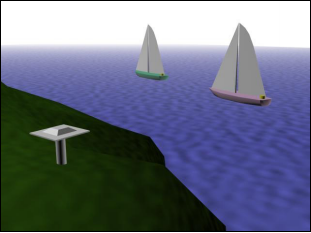
\includegraphics [scale=0.6] {single_positioning}
  \caption{Single режим. Корабли в роли роверов не используют базу, установленную на берегу}
  \label{img:latex}
\end{figure}

Изображенные на рисунке 1.2 Kinematic и Static режимы отвечают за стандартную RTK функциональность. Сырые данные ровера совмещаются с сырыми данными базовой станции, находящейся в заранее известной позиции для получения уточненной позиции ровера. Режим Kinematic подразумевает, что ровер находится в движении и является наиболее используемым. Static подразумевает, что ровер не двигается. Для работы в таком режиме между ровером и базой требуется постоянная связь для передачи поправок. В таком режиме ровер также позволяет писать логи, причем отдельный для сырых данных ровера и отдельный для полученных поправок. Это может быть очень полезно для определения проблем, касающихся связи между двумя приемниками.

\begin{figure}[ht]
  \center
  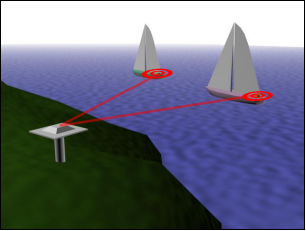
\includegraphics [scale=0.6] {static_kinematic_positioning}
  \caption{Static и Kinematic режимы. Корабли в роли роверов получают поправки от базы, установленной на берегу}
  \label{img:latex}
\end{figure}

Режим Moving-Baseline \cite{trimble-rtk} гораздо менее распространен, однако не менее интересен(рис. 1.3). Принцип несколько отличается от Kinematic. Главная идея – движущаяся база. Такой режим не позволяет получить значительно лучшую абсолютную точность, однако относительно друг друга пара приемников получает крайне точные координаты. Также данный режим можно использовать как GPS компас.

\begin{figure}[ht]
  \center
  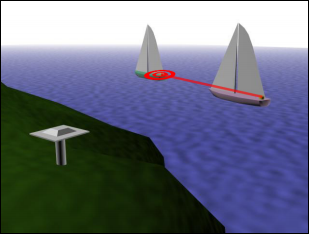
\includegraphics [scale=0.6] {movingbase_positioning}
  \caption{Moving-Baseline режим. Один из движущихся кораблей выполняет роль ровера, другой базы}
  \label{img:latex}
\end{figure}

PPP(Precise point positioning) режимы используются в первую очередь как подготовка к основной работе в режиме RTK. Например, PPP-Static можно использовать для определения положения будущей базы. Суть работы в таком режиме – накопление и усреднение информации о позиции приемника. Таким образом, проработав несколько часов на одной точке, приемник сможет с хорошей степенью точности определить координаты этой точки, и эти данные можно использовать для настройки базы.

\subsection{Форматы данных} \label{subsect_1_2_3}

RTKLIB поддерживает большое количество форматов хранения данных, так или иначе связанных с ГНСС навигацией. Этот набор включает как независимые от приемника форматы, например RINEX, так и проприетарные протоколы, используемые приемниками для выдачи координат.

Стандартные форматы включают в себя RINEX, RTCM, NMEA. RINEX, или Receiver Independent Exchange Format, является стандартом для хранения любых навигационных данных и поддерживается большинством геоинформационных систем. RTCM(Radio Technical Commission for Maritime Services) – формат, полностью нацеленный на увеличение скорости передачи данных. В первую очередь используется для передачи поправок с базы. NMEA(National Marine Electronics Association) – один из самых популярных форматов, поддерживается повсеместно, отличается от RTCM тем, что он текстовый.

Среди проприетарных протоколов следует выделить крайне популярный UBX, так как приемники компании u-blox широко используются в различных областях, от телефонов до беспилотников, и относительно дешевы. Кроме этого, поддерживаются приемники NovAtel, Hemisphere, JAVAD, Furuno и NVS.

\subsection{Обзор программ в составе пакета RTKLIB} \label{subsect_1_2_4}

Чтобы получить некоторое представление о внутреннем устройстве, а также о разделении обязанностей внутри проекта, следует рассмотреть основные программы, входящие в RTKLIB. На данный момент, в версии 2.4.2 их семь: RTKPLOT, RTKCONV, STRSVR, RTKPOST, NTRIP Browser, RTKNAVI и RTKGET. Следует подробно рассмотреть три из них, отвечающие за основные функции - RTKNAVI, STRSVR и RTKCONV.

\subsubsection{RTKNAVI} \label{subsubsect_1_2_4_1}

\begin{figure}[ht]
  \center
  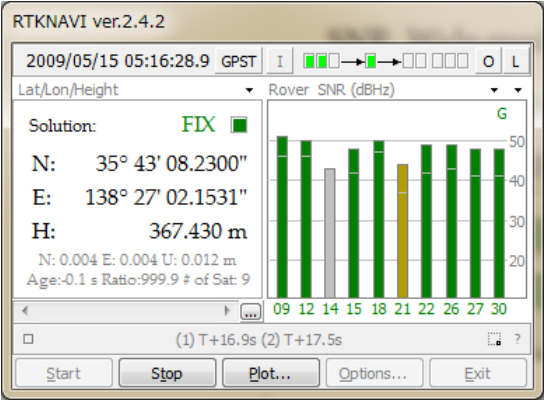
\includegraphics [scale=0.6] {RTKNAVI_screenshot}
  \caption{RTKNAVI}
  \label{images:latex}
\end{figure}

RTKNAVI – основная программа, выполняющая RTK функции. По сути, именно RTKNAVI выполняет все обязанности ровера. В эти задачи входит:

\begin{enumerate}
  \item Принять сырые данные с приемника ровера;
  \item Принять поправки с базы;
  \item Опционально, записать эти данные в лог;
  \item Применить к этим данным RTK алгоритм;
  \item Полученное решение сделать доступным в нескольких форматах на выбор.
\end{enumerate}

RTKNAVI также показывает информацию о качестве текущего решения, уровни приема сигнала спутников базы и ровера. RTKNAVI имеют версию с интерфейсом командной строки - \textbf{RTKRCV}. RTKRCV запускается под GNU/Linux и имеет ту же функциональность, что и RTKNAVI. Текстовая версия так же может показать статус RTK решения, координаты и информацию о приеме спутников. Однако, если графическая версия имеет отдельное окно с настройками, то RTKRCV настраивается с помощью конфигурационных файлов. Работа с ними может быть сложна и требует серьезного навыка.

\subsubsection{STRSVR} \label{subsubsect_1_2_4_2}

\begin{figure}[ht]
  \center
  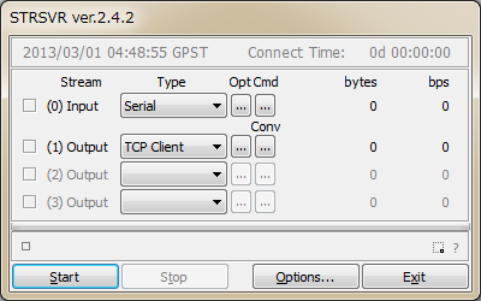
\includegraphics [scale=0.6] {STRSVR_screenshot}
  \caption{STRSVR}
  \label{img:latex}
\end{figure}

STRSVR – мультиплексор потоков. Позволяет перенаправить данные подключенного к компьютеру приемника в три новых потока. Среди возможных каналов приема и отправки данных есть COM-порты, TCP сокеты, файлы, HTTP и FTP протоколы, а также NTRIP протокол, часто используемый базовыми станциями для передачи данных через интернет. Кроме того, STRSVR - единственная программа в пакете, способная выдавать легковесный RTCM3, поэтому по умолчанию используется для обеспечения функциональности базы. Текстовая версия носит название \textbf{STR2STR}.

% \clearpage

\subsubsection{RTKCONV} \label{subsubsect_1_2_4_3}

\begin{figure}[ht]
  \center
  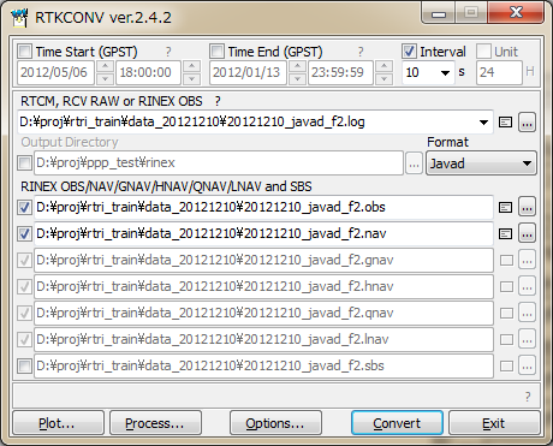
\includegraphics [scale=0.6] {RTKCONV_screenshot}
  \caption{RTKCONV}
  \label{img:latex}
\end{figure}

Универсальный конвертер спутниковых данных из одного формата в другой. Наиболее важное применение – перевод логов из форматов, связанных с приемником, например UBX, в независимый RINEX для дальнейшего анализа и пост-обработки. RTKCONV имеет текстовую версию, называемую \textbf{CONVBIN}.

\section{Проблемы в использовании RTKLIB} \label{sect1_3}

Несмотря на свои обширные возможности и открытый исходный код, RTKLIB - слабораспространенный и малоизвестный программный комплекс. Это связано в первую очередь не с качеством получаемых результатов, а с удобством использования.

Графические версии приложений запускаются только под ОС семейства Windows. Однако, технология RTK по-настоящему раскрывает свой потенциал при интеграции в технику. А, так как встраивать, например в беспилотник, полноценный ноутбук проблемно, гораздо большую популярность имеет версия с интерфейсом командной строки. \textbf{RTKRCV} - программу, отвечающую за расчет RTK решения в реальном времени можно запускать на практически любой платформе под управлением GNU/Linux. Код написан на языке C, и RTKRCV не требует больших ресурсов, несмотря на большое количество вычислений. Тем не менее, чтобы работать с системой, в том числе запускать и останавливать расчеты, нужен постоянно открытый терминал, а соответственно полноценный компьютер с клавиатурой и доступу к данным с приемника.

Так как RTKLIB - крайне многофункциональный комплекс ПО, а обилие настроек, несколько принципиально отличающихся режимов работы и неочевидные решения в дизайне путают как новичка, так и опытного пользователя, порог вхождения очень высок. Более того, текстовая версия настраивается с помощью конфигурационных файлов, состоящих из примерно ста двадцати параметров. Без подсказок опытного пользователя, сдвинуться с места при освоении этого ПО очень сложно.

Чтобы обойти эти ограничения, предлагается добавить на вычислительный модуль, встроенный, например в автомобиль, еще одно приложение помимо RTKRCV. Задачей данного приложения будет обмен информацией и командами между RTKRCV и веб-страницей. Таким образом, для проверки статуса или изменения настроек можно будет использовать любое устройство с браузером, например смартфон.

\section{Платформа для разработки} \label{sect1_4}

В качестве платформы для разработки и тестирования будет использоваться Emlid Reach \cite{reach-docs}. Reach представляет с собой составное устройство, состоящее из вычислительного модуля Intel Edison и дополнительной платы, на которой стоит ГНСС приемник компании u-blox. На борту Intel Edison - Linux, что делает это полностью подготовленной для работы средой - возможности запустить RTKLIB, наличия Python и менеджера пакетов PIP достаточно для разработки.

\begin{figure}[ht]
  \center
  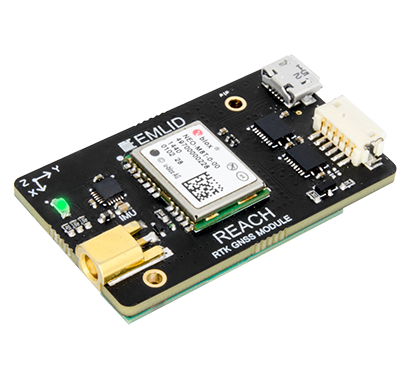
\includegraphics [scale=0.6] {emlid_reach}
  \caption{Emlid Reach}
  \label{img:latex}
\end{figure}

\section{Примеры веб-интерфейсов для работы с устройствами} \label{sect1_5}

Наиболее распространенным примером веб-интерфейса для ПО, работающего на устройстве без основных органов управления являются современные маршрутизаторы. Почти у всех современных моделей, с незначительными отличиями, присутствует проприетарный интерфейс, работающий именно по такой схеме. В последнее время популярность набирает дистрибутив GNU/Linux, созданный специально для маршрутизаторов - OpenWrt. Для сравнения возьмем новую версию Windows 10 для встраиваемых устройств.

\subsection{OpenWrt LuCI} \label{subsect_1_5_1}

Рассмотрим примеры того, как реализован веб-интерфейс LuCI \cite{luci-docs}, являющийся лицом OpenWrt. Первое, что следует заметить в организации интерфейса(рис. 1.5) - верхнее меню с разделением всех страниц на несколько категорий - Status, System, Network. За каждой из кнопок скрывается выпадающее меню с несколькими подкатегориями.

Основная задача LuCI - настройка устройства. Для этого отлично подходят гибкие веб формы.

\begin{figure}[ht]
  \center
  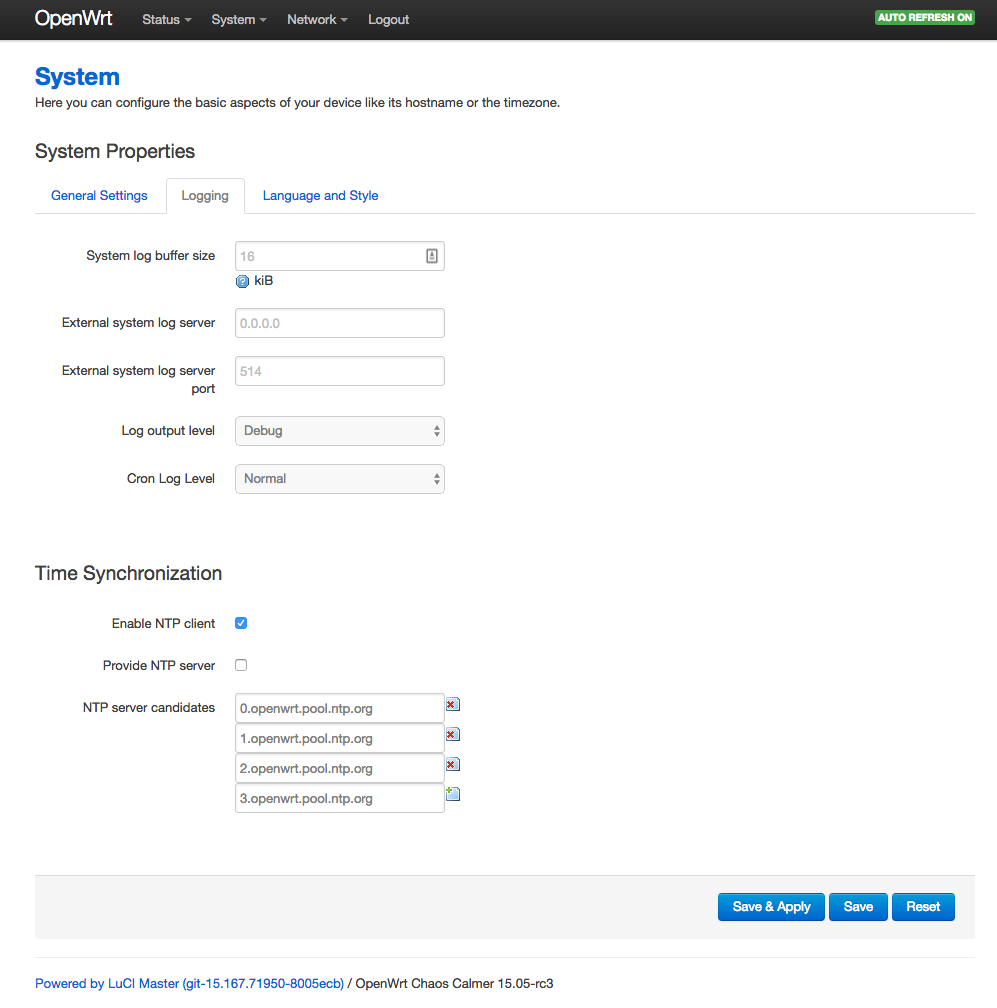
\includegraphics [scale=0.3] {OpenWrt_logging}
  \caption{Настройки системного логгирования в OpenWrt}
  \label{img:latex}
\end{figure}

Хороший пример - внутренние настройки логгирования маршрутизатора. Легко заметить разнообразие используемых элементов: текстовые формы с предлагаемыми значениями, выпадающие списки, флажки.

Кроме этого, интересна возможность наблюдать за загрузкой сети с помощью графиков(рис. 1.6). Это гораздо более наглядное представление информации, чем простой текст. Веб-технологии позволяют сделать график отзывчивым и «живым» без особого труда.

\begin{figure}[ht]
  \center
  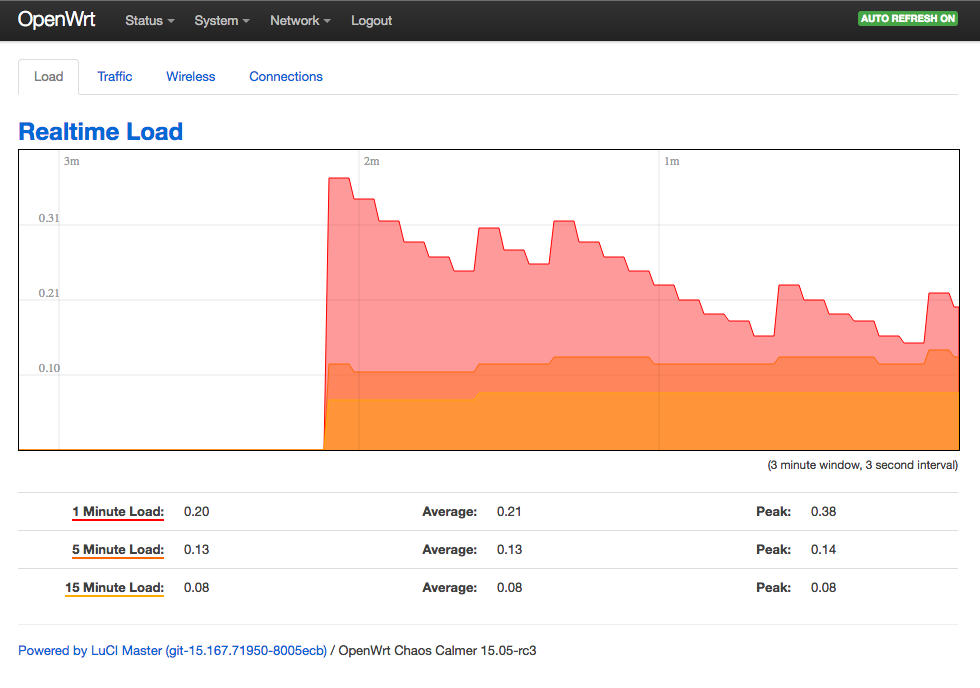
\includegraphics [scale=0.3] {OpenWrt_netgraph}
  \caption{График загрузки сети в OpenWrt}
  \label{img:latex}
\end{figure}

\clearpage

\subsection{Microsoft Windows 10 IoT Core} \label{subsect_1_5_2}

Вместе с выпуском Windows 10, Microsoft выпустила новую, урезанную версию ОС, специально для маленьких устройств без встроенных экрана или клавиатуры, таких как Raspberry Pi и MinnowBoard Max. Версия Windows 10 IoT Core \cite{windows-docs} также использует веб-страницу для взаимодействия с пользователем(рис 1.7).

\begin{figure}[ht]
  \center
  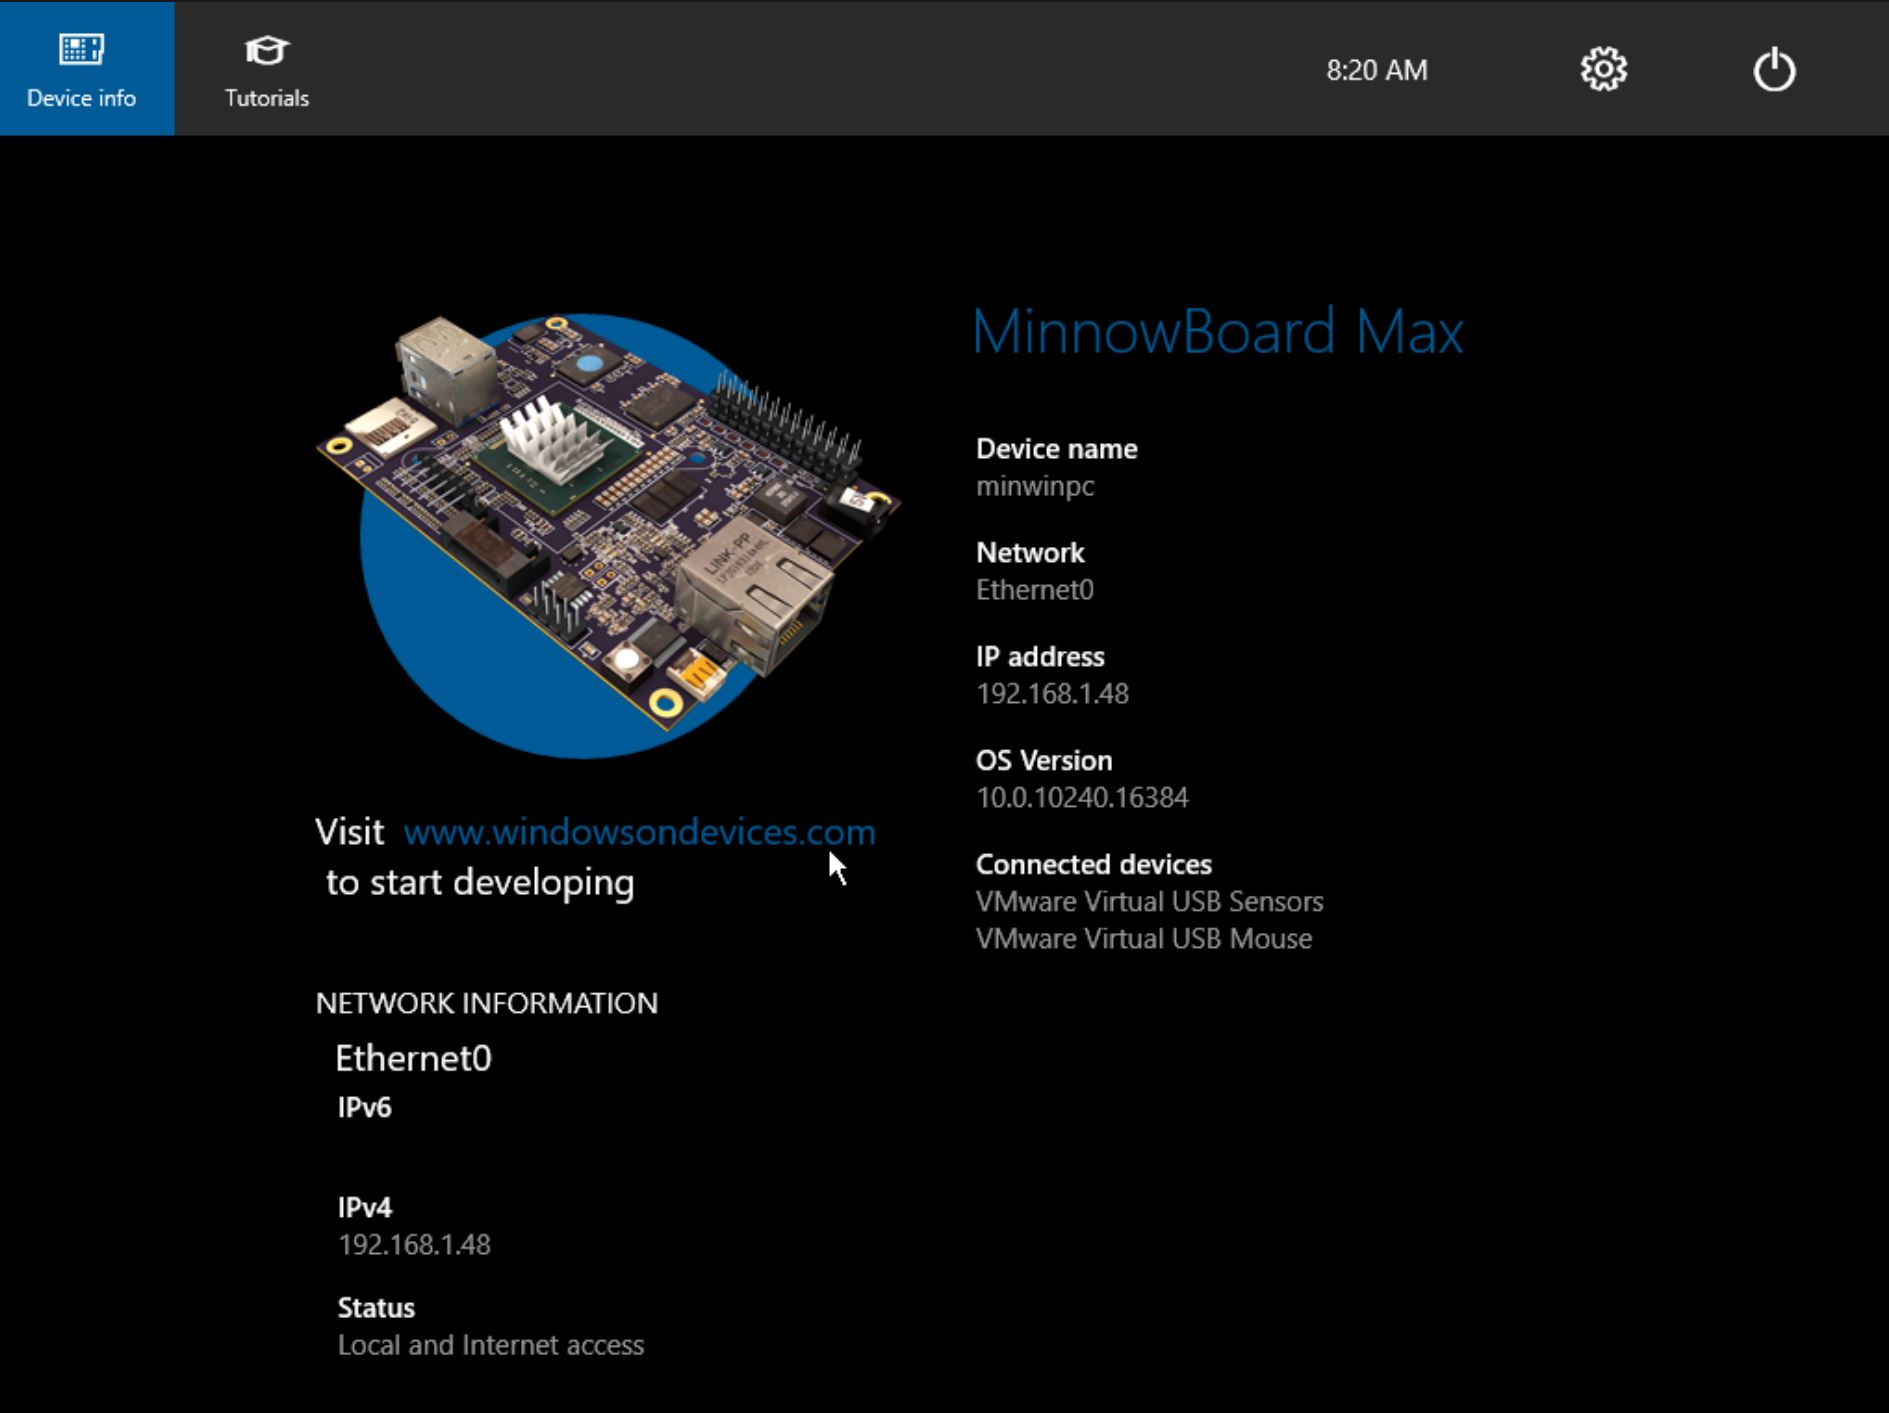
\includegraphics [scale=0.5] {Win10_deviceinfo}
  \caption{Главный экран Windows 10 IoT Core}
  \label{img:latex}
\end{figure}

% \clearpage

На рисунке 1.8 изображен  менеджер подключенных устройств. Веб-технологии позволяют создать адаптивный интерфейс в виде раскрывающегося списка распознанных устройств.

\begin{figure}[ht]
  \center
  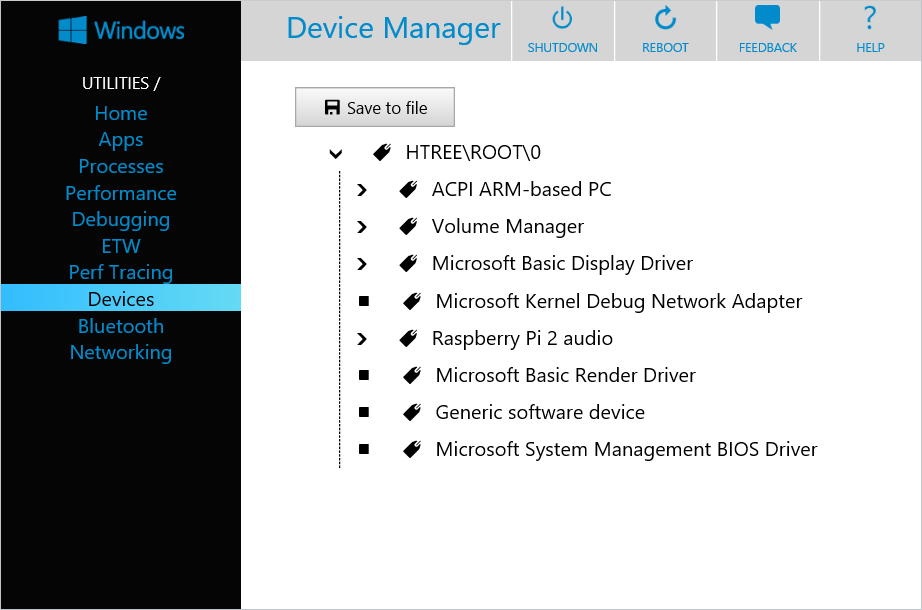
\includegraphics [scale=0.3] {Win10_settings}
  \caption{Менеджер устройств Windows 10 IoT Core}
  \label{img:latex}
\end{figure}

\section{} \label{sect1_6}













